\chapter{general framework of the project}
\section*{Introduction}
Ensuring the smooth launch and ongoing availability of crucial applications is vital for businesses in today's digital landscape. This project outlines a strategic approach to achieve this goal by streamlining deployment processes and minimizing downtime.
\par
We will implement detailed plans for launching each application, including clear timelines, defined responsibilities, and contingency measures to address potential risks and disruptions. This will ultimately enhance the stability and performance of our key applications, contributing to overall business success.
\section{The Host Organization}
\paragraph[short]{ADACTIM}
is a Managed Services Operator specializing in the Cloud, application integration and outsourcing, ERP and BI, operating internationally via a presence in Europe, the Maghreb and Africa.
\newline
this figure \ref{fig:logo_Adactim} present the logo of the company.

\begin{figure}[htpb]
    \centering
    \frame{
\includegraphics[width=0.5\columnwidth]{logo-adactim.png}}
    \caption{Logo Entreprise Adactim}
    \label{fig:logo_Adactim}
\end{figure}

\subsection*{Adactim  Mission}
ADACTIM enables the company to benefit from technological transformations in the areas of IT infrastructure and integrated business systems allowing it to focus its energy on its core business.
\par
Our mission is to facilitate businesses' access to technological innovations, to simplify their daily use, allowing the company to be more efficient and competitive.
\par
Our company focuses its resources on its development and its customers. To that end, the company should be well-equipped with business software and IT infrastructure and outsource appropriate operations processes.
\section{Existing study}

\noindent
\textbf{Description of the Current Environment:}
\\
Our core business application currently runs on a manually provisioned Azure cloud infrastructure managed through the web portal.
\\
\textbf{Analysis of Existing Deployment Processes:}

\begin{figure}[htpb]
    \centering
    \frame{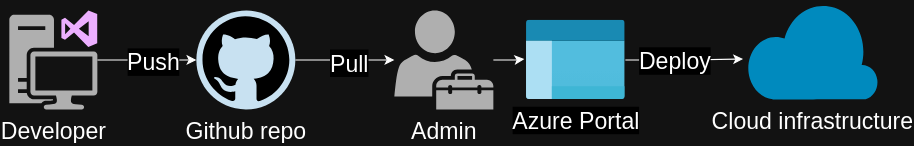
\includegraphics[width=0.8\columnwidth]{existing_stratigy.png}}
    \caption{existing strategy of the application deployment}
    \label{fig:existing_strategy}
\end{figure}

The deployment of applications in our current setup involves several steps, including code preparation, testing, deployment scheduling, and monitoring. Each deployment requires coordination between multiple teams, including developers, quality assurance, and system administrators.
Strengths and Weaknesses of the Current Approach:
\\
\textbf{Strengths:}
\begin{itemize}
    \item Our current deployment process follows a structured workflow, ensuring thorough testing before releasing applications into production.
    \item Effective communication and collaborative problem-solving are facilitated by teamwork during deployments.
\end{itemize}
\textbf{Weaknesses:}
\begin{itemize}
    \item Extended outages caused by inefficient deployment practices negatively impact business continuity and revenue.
    \item Limited automation in certain areas leads to manual errors and delays during deployments.
\end{itemize}

\section{Problematic}
While our current deployment process prioritizes rigorous testing and cross-team collaboration, it faces significant challenges impacting both efficiency and reliability. One critical issue lies in the protracted nature of deployment timelines. This stems from the inherent complexity of coordinating and executing numerous manual testing processes. Consequently, not only are the releases of crucial applications delayed but the potential for human error during manual interventions is also amplified
\par
In essence, our current application deployment process faces a critical challenge: balancing the strengths of its structured workflow and collaborative approach with the need for faster, more automated deployments.

\section{Needs and requirements}
\noindent
\textbf{Functional Needs:}
\begin{itemize}
    \item \textbf{Patch Deployment Automation:} Implement a system for automated deployment of patches to applications and systems.
    \item \textbf{Version Rollback Capability:} Provide the ability to revert to a previous version of an application during deployment in case of failure or unexpected issues.
\end{itemize}
\textbf{Non-functional Needs:}
\noindent
\begin{itemize}
    \item \textbf{Availability:} Ensure high availability of applications and services, minimizing downtime during deployments.
    \item \textbf{Security:} Implement Web Application Firewall (WAF) and Container Application Firewall (CAF) to safeguard applications and containers from cyber threats.
    \item \textbf{Performance:} Optimize deployment processes to maintain optimal performance levels of applications and systems.
    \item \textbf{Cost optimization:} Minimize the costs associated with deployment processes, including recourses and infrastructure.
\end{itemize}

\section{Proposed Deployment Optimization Solution}
In order to address the identified challenges and meet the outlined needs and requirements, we propose a solution that leverages modern technologies and methodologies.
\begin{itemize}

    \item \textbf{Provisioning and Configuration Management:}
          Automate the provisioning and configuration of cloud infrastructure and application environments to ensure consistency and reliability using Infrastructure as Code (IaC) and Configuration Management tools.

    \item \textbf{Automating the build and testing process:}
          To minimize manual intervention and expedite development cycles, let's leverage automation across the build and testing pipeline. This not only reduces human error but also frees up valuable time for developers to focus on core tasks.
    \item \textbf{implementing a Deployment strategy:}
          Implement a deployment strategy that leverages automation to ensure seamless and efficient application deployments, minimizing downtime and errors. By applying these pattern principles:
          \begin{itemize}
              \item \textbf{central secrets store:}storing and monitoring the secrets that our application needs. We will use Azure Key Vault to implement this pattern.
              \item \textbf{Rightsize resources for each environment:} ensuring that the resources allocated to each environment are appropriate for the expected load. We can do this by implementing workspaces in Terraform.
              \item \textbf{Delete non-production environments:} ensuring that non-production environments are deleted when they are no longer needed.
              \item \end{itemize}
\end{itemize}


\section{Objectives}
throughout  this project we will adopt the scrum methodologies to achieve the following objectives:
\begin{longtable}[c]{
    |p{.20\textwidth}
    |p{.55\textwidth}|
    p{.21\textwidth}|
    }
    \caption{the key technical objectives for the project}
    \label{tab:objectivesTable}                      \\
    \hline

    the Sprints
     & Objectives
     & Delivrables                                   \\
    \hline

    Sprint1(2 weeks)
     & Probision the cloud infrastructure as IaC
     & Terraform scripts                             \\
    \hline

    Sprint2(2 weeks)
     & Implement the Continuous Integration pipeline
     & a DevOps workflow                             \\
    \hline

    Sprint3(2 weeks)
     & Set up a deployment strategy
     & seamless deployment                           \\
    \hline

    Sprint4(1 week)
     & Optimization and cost reduction
     & cost reduction report                         \\
    \hline

    Sprint5(1 week)
     & Write the necessary documentation
     & Documentation                                 \\
    \hline
\end{longtable}

\section{Methodology of the project}
While some projects might seem straightforward, a defined methodology is crucial for achieving success.  This framework provides a roadmap, ensuring tasks are completed efficiently and in the right order. By following a methodology, you can avoid common pitfalls, manage your time effectively, and ultimately deliver a successful project.
\subsection*{choice of the Agile methodology}
While seemingly designed for larger teams, Agile methodologies\cite{webArticle0} offer valuable structure even for single-person projects. Their core principles of iterative development, continuous improvement, and flexibility empower individuals to efficiently manage projects and adapt to changing requirements.
Let's explore some popular Agile methodologies and their strengths:
\begin{itemize}
    \item \textbf{scrum:} Scrum is an agile framework that helps teams structure their work into short development cycles called sprints. Scrum teams commit to shipping work at the end of each sprint and adopt practices and a team structure that helps them achieve this cadence. Scrum takes the agile principles one step further, creating structure that helps teams live the agile principles in their day-to-day work. Scrum is a well-documented agile framework that many teams can adopt without much disruption.
    \item \textbf{Kanban:} To master Kanban, you need to be familiar with four essential Kanban metrics—lead time, cycle time, work-in-progress, and throughput. That means that implementing kanban will introduce an additional overhead to the project.
    \item \textbf{Waterfall:} Waterfall delivery is focused on the development of products or solutions based on specifications from the client or business. Teams study the requirements and build the solution over weeks, months, or even years. Waterfall is the preferred method in regulated industries where tolerances are very narrow.
\end{itemize}
\subsection*{Verdict:}
Considering the project's potential for evolving requirements and the benefits of iterative development, Scrum emerges as the optimal choice. Its focus on defined sprints, adaptability, and a structured approach to project management, even for solo developers, aligns perfectly with our project needs.

\section*{Conclusion}
This chapter outlined the challenges associated with our current application deployment process, which prioritizes thorough testing and collaboration but suffers from lengthy timelines and manual errors. To address these shortcomings, we proposed a new approach that leverages modern technologies and methodologies to achieve faster, more reliable deployments.
\par
The proposed solution emphasizes automation throughout the deployment lifecycle, encompassing infrastructure provisioning, build and testing processes, and the deployment strategy itself. This will minimize manual intervention, reduce errors, and expedite deployments. Additionally, the strategy incorporates security best practices and performance optimization techniques to ensure the applications' continued reliability and availability.
\par
The next chapter, "Detailed Existing Study," delves deeper into the technical underpinnings of our current environment. It provides a comprehensive analysis of the existing architecture and deployment process, laying the groundwork for the implementation of the proposed optimization solution in subsequent chapters.